\documentclass[a4paper,parskip=half-]{scrartcl}
\usepackage[utf8]{inputenc}
\usepackage[english]{babel}
\usepackage{fancyhdr}
\usepackage{graphicx}
\usepackage{hyperref}
\usepackage{amsmath}
\graphicspath{{c://users//fmeyer//git//ml_ss20/files/graphics/}}

\pagestyle{fancy}
\fancyhf{}
\rhead{
	\small 
		\begin{tabular}[t]{l}
		\textsf{Fabian Meyer, 6816480}\\
		\textsf{\url{https://github.com/gitfabianmeyer/ml_ss20}}
		\end{tabular}}
\lhead{Machine Learning}



\begin{document}
	\section{Stochastic Gradient Descent}
	In this exercise we solved the stochastic gradient descent algorithm for a regression problem.\\
	The problem consists of 100 artificial data points, following a sinus curve with random noise in the interval $[-0.3,0.3]$. The initial parameter of the polynomials are random generated in the interval $[-0.5,0.5]$.\\
	In the experiments, I utilized the learning rates $\alpha \in [0.001,0.01,0.05,0.1,0.15,0.2,0.3,0.5,1]$ and $D \in [1,2,3,4]$, running the model for 14.000 iterations each.
	\subsection{Final Model}
	
	The best model, measured in root-mean-squared-error $$E_{RMS} = \sqrt{2E(\theta)/m}$$ 
	where  $$E(\theta) = \frac{1}{2}\sum^{m}_{i=1}(h_{\theta}(x_i) - y_i)^2$$
	was performed by a model with learning rate $\alpha = 0.1$ and $D=4$ with the polynomial\\
	\begin{align*}
		h_{\theta}(x) &= 0.05399324797581987 + 8.800521038331368x -23.000200637422502x^2 \\&+ 7.542748857562933x^3 +6.734454552273191x^4
	\end{align*}
	The resulting error was $E_{RMSE} = 0.18234297782816197$. The plotted curve and the error curve are plotted in subsection \ref{plots}. You can see that the resulting curve is slightly different from the original sinus curve, which is most likely caused by the low number of data points and the random noise. For a higher number of data points, e.g. 1.000.000, the fitted model will probably converge to the original sinus curve, following the law of large numbers.
	\subsection{Plots}\label{plots}
	\begin{figure}
	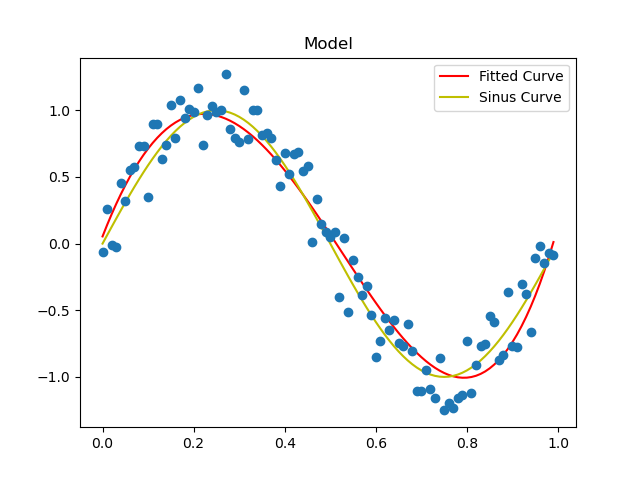
\includegraphics{model_ex1}
	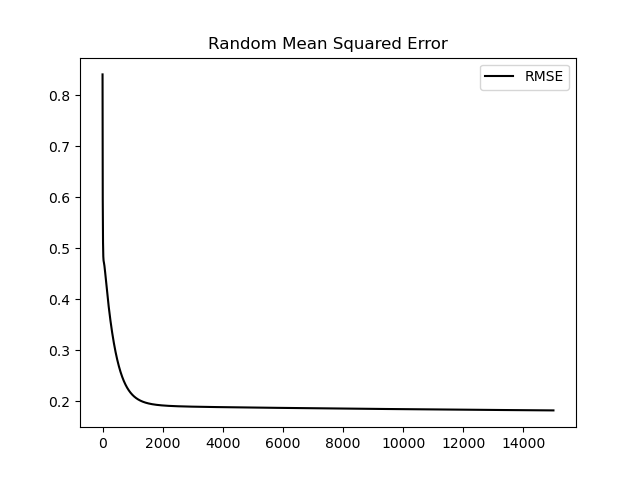
\includegraphics{RMSE_ex1}
	\end{figure}

\end{document}
